\section{Customer relationship management}\label{sec:appendix01}

\subsection{CRM notions}
\label{app:crm}
brenneckes crm defs und so 
Appendices provide only two structural levels, \viz, \texttt{\textbackslash section}, and \texttt{\textbackslash subsection}.

Search on scopus, queries are column headings searched in title, abstract and keywords. 

\begin{table}[caption={CRM publication comparison}, label=tab:crmnotioncomparison]
	\centering

	\begin{tabular}{p{1cm}| p{2cm} |p{4.3cm}|p{3cm}   } 
		\textbf{Year} & \textbf{"CRM"} & \textbf{"Customer relationship management"} & \textbf{"Customer Management"} \\ \hline 
		2016          & 211            & 34                                          & 8                              \\
		2015          & 198            & 32                                          & 5                              \\
		2014          & 178            & 35                                          & 4                              \\
		2013          & 193            & 37                                          & 2                              \\
		2012          & 166            & 40                                          & 5                              \\
		2011          & 138            & 44                                          & 7                              \\
		2010          & 131            & 32                                          & 1                              \\
		2009          & 133            & 27                                          & 6                              \\
		2008          & 99             & 22                                          & 2                              \\
		2007          & 118            & 26                                          & 1                              \\
		2006 & 111          & 19                           & 1									 \\
	\end{tabular}
\end{table}

\subsection{Multi- and Omni-channel}
\label{app:mcoc}
The search is done on scopus and queries are \enquote{TITLE-ABS-KEY ( ( omnichannel  OR  omni-channel )  AND  ( crm  OR  management  OR  retail )  AND  customer )} and \enquote{TITLE-ABS-KEY ( ( multichannel  OR  multi-channel )  AND  ( crm  OR  management  OR  retail )  AND  customer )}, respectively.

\begin{table}[caption={multi- and omni-channel publication comparison}, label=tab:crmnotioncomparison]
	\centering
	\begin{tabular}{p{1cm}| p{2cm} |p{4.3cm}|p{3cm}   } 
	\textbf{Year} & \textbf{"Multi-channel"} & \textbf{"Omni-channel"} \\ \hline 
	2016          & 32            & 15                                                                       \\
	2015          & 33            & 10                                                                   \\
	2014          & 30            & 7                                                                   \\
	2013          & 17            & 1                                                           \\
	2012          & 24            & 1                                                              \\
	2011          & 24            &                                                       \\
	2010          & 25            &                                                                \\
	2009          & 34            &                                                       \\
	2008          & 29             &                                             \\
	2007          & 23            &                                                       \\
	2006 & 29         &                           					 \\
\end{tabular}
\end{table}


\subsection{Outsourcing provider processes}
\label{app:provproc}

		\begin{figure}[caption={Outsourcing provider processes}, label={fig:scheweproc}]
	{	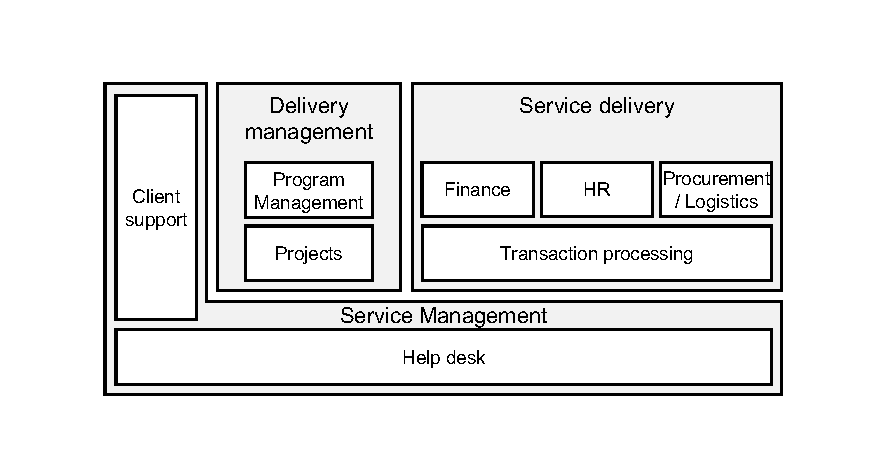
\includegraphics[width=.8\textwidth]{figures/scheweproc.pdf}}
		\hspace{6.2cm}	SOURCE: \citep[\p{98}]{schewe2007}
\end{figure}
\subsection{Selected reference models}
\label{app:refmods}
	\begin{figure}[caption={SCOR Model}, label={fig:scor}]
	{	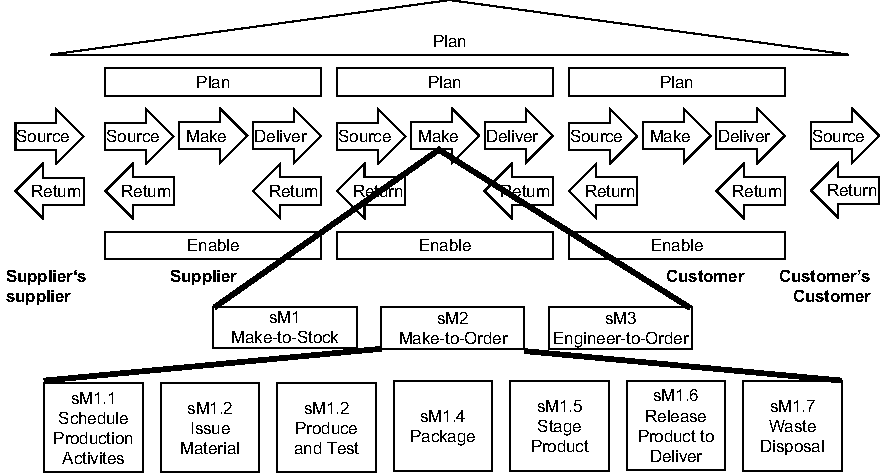
\includegraphics[width=.8\textwidth]{figures/scor.pdf}\\
	\quelle{\citep{APICS2015}}} 
\end{figure}

	\begin{figure}[caption={Retail-H}, label={fig:retailh}]
	{	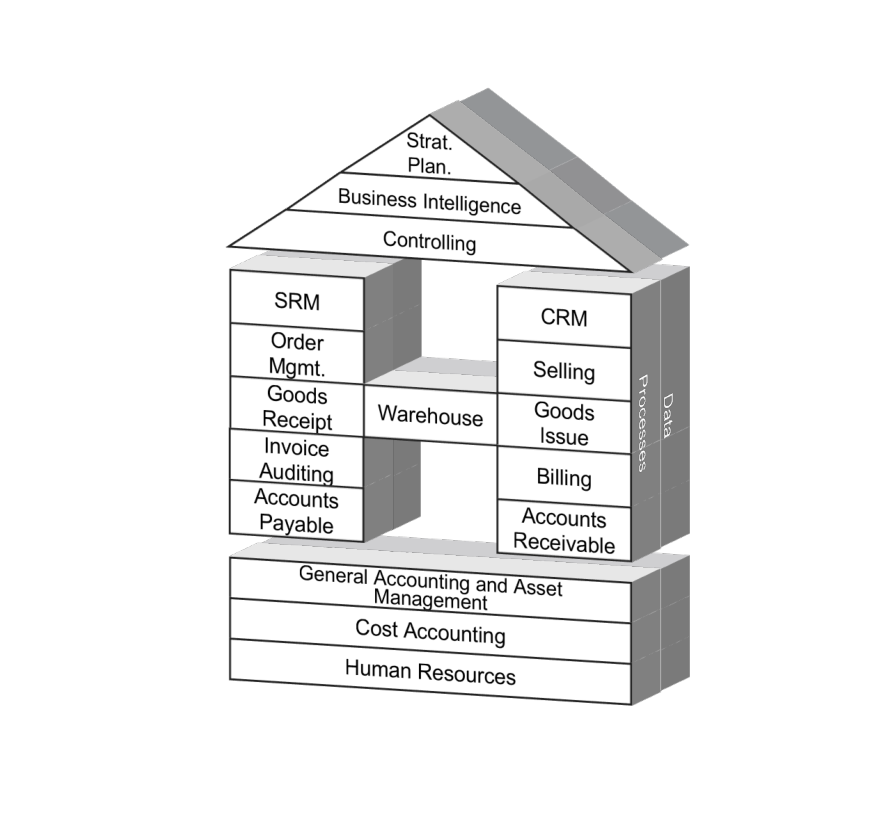
\includegraphics[width=.6\textwidth]{figures/retailh.pdf}
	\\
\quelle{\citep{becker2004handelsinformationssysteme}}}
	
\end{figure}

\subsection{Some Appendix Subsection}

\lipsum[10]